
%(BEGIN_QUESTION)
% Copyright 2012, Tony R. Kuphaldt, released under the Creative Commons Attribution License (v 1.0)
% This means you may do almost anything with this work of mine, so long as you give me proper credit

An interesting type of AC motor is the {\it wound-rotor} motor.  The stator of a wound-rotor machine is identical to the stator of any three-phase induction motor: sets of windings connected together in either a ``wye'' or a ``delta'' configuration, powered by a three-phase AC source.  

However, the rotor of a wound-rotor maching is quite different from the rotor of a squirrel-cage machine.  Instead of rotor bars short-circuited together by shorting rings as in the case of a squirrel-cage induction motor, the wound-rotor induction motor has copper wire windings on the poles of the rotor, connected to a pair of slip rings contacting stationary carbon brushes, allowing an external circuit to be connected to the rotor coil:

$$\includegraphics[width=15.5cm]{i01231x01.eps}$$

When this external circuit is open, the motor will not spin.  When this circuit is short-circuited, the motor acts the same as a squirrel-cage induction motor.  When this circuit is energized with direct current (DC), the motor becomes a {\it synchronous} motor.

\vskip 10pt

Explain how this one motor is able to operate in these different modes, appealing to general principles of AC motors such as Lenz's Law.  Also, identify how this motor would operate if an electrical resistance were connected between the two brush terminals, rather than being open-circuited, short-circuited, or DC-energized.

\vskip 20pt \vbox{\hrule \hbox{\strut \vrule{} {\bf Suggestions for Socratic discussion} \vrule} \hrule}

\begin{itemize}
\item{} Identify a practical purpose for a wound-rotor motor.
\end{itemize}

\underbar{file i01231}
%(END_QUESTION)





%(BEGIN_ANSWER)

If a resistance is connected within the rotor circuit, the motor will behave as a ``weak'' induction motor: spinning slower and with less torque than it will with a short-circuited rotor winding.  For this reason, wound-rotor induction motors were once popularly used for variable-speed applications: the speed and torque of the motor could be easily varied simply by connecting different values of resistors within the rotor circuit!
 
\vskip 10pt

With the rotor winding open-circuited, there is no path for current within the rotor winding.  This means Lenz's Law will have no effect, because there will be no induced {\it current} within the rotor winding (although there will certainly be an induced {\it voltage}!).  With no induced rotor current, there will be no torque exerted on the rotor, and therefore the rotor will not spin.

\vskip 10pt

With the rotor short-circuited, it will be equivalent to the permanently short-circuited rotor of a ``squirrel-cage'' induction motor, and therefore will act just the same.

\vskip 10pt

With the rotor winding energized by DC, it will have a definite magnetic polarity and will therefore attempt to follow the stator's rotating magnetic field in lock-step.


%(END_ANSWER)





%(BEGIN_NOTES)


%INDEX% Electronics review: wound-rotor induction motor operation

%(END_NOTES)


